\documentclass[aspectratio=169,10pt]{beamer}
\usepackage[utf8]{inputenc}
\usepackage[T2A]{fontenc}
\usepackage[russian]{babel}
\usepackage{amsmath}
\usepackage{booktabs}
\usepackage{graphicx}

\usetheme{Madrid}
\usecolortheme{default}
\setbeamertemplate{navigation symbols}{}
\setbeamertemplate{caption}[numbered]
\graphicspath{{figs/}}

\newcommand{\Nt}{\mathrm{N_2}}

\title[Низкотемпературная плазма]{Генерация и исследование свойств\\
  низкотемпературной плазмы субатмосферного давления}
\subtitle{Лабораторная работа №\,19}
\author[Ларькин Г.]{Ларькин Глеб, Б03-301}
\institute[МФТИ]{МФТИ, Физтех-школа аэрокосмических технологий}
\date{2026}

\begin{document}

% ---------------------------------------------------------------
\begin{frame}
  \titlepage
\end{frame}

\begin{frame}{Цели и задачи}
  \textbf{Два способа получить неравновесную плазму при $P_m \sim 1$--10~Торр}
  \begin{enumerate}
    \item \textbf{Электронно-пучковая плазма (ЭПП):} пучок 30~кэВ в
          кварцевой трубке с $\Nt$ и Ar при 1; 2,5; 5~Торр
          \begin{itemize}
            \item профили свечения $B(z)$ по фотографиям
            \item расчёт энерговыделения $Q(z)$ методом Монте-Карло, сравнение
          \end{itemize}
    \item \textbf{ВЧ-ёмкостный разряд} (13,56~МГц) в чистом и техническом гелии
          \begin{itemize}
            \item профили $I(L)$, переход $\alpha\to\gamma$, величина $P_m L$
            \item спектроскопия: состав плазмы, доля примеси $\Nt$
            \item оптическая прозрачность плазмы
          \end{itemize}
  \end{enumerate}
\end{frame}

% ===============================================================
\section{Электронно-пучковая плазма}
% ===============================================================

\begin{frame}{ЭПП: установка}
  \begin{columns}[T]
    \begin{column}{0.55\textwidth}
      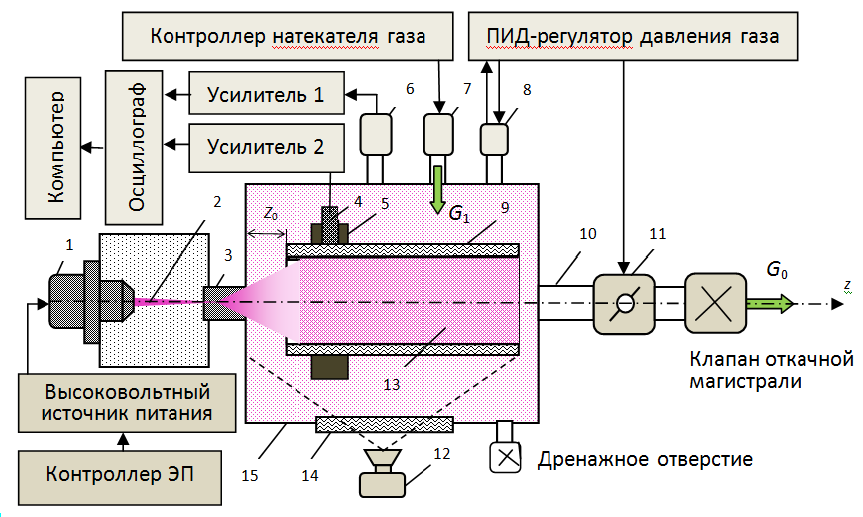
\includegraphics[width=\linewidth]{scheme_epp.png}
    \end{column}
    \begin{column}{0.43\textwidth}
      \small
      \begin{itemize}
        \item триодная пушка, катод LaB$_6$, вакуум $10^{-5}$~Торр
        \item $E_b = 30$~кэВ, $I_b = 2$--4~мА
        \item ввод в газ через \textbf{газодинамическое окно}
        \item кварцевая трубка: 310~мм, $\varnothing 24{,}8$~мм
        \item давление: ПИД-регулятор + баратрон
        \item CCD-камера через смотровое окно
      \end{itemize}
      \medskip
      \textbf{Гипотеза:} свечение $B \propto Q_\text{ex}$ ---
      скорости возбуждения, т.\,е. энерговыделению пучка
    \end{column}
  \end{columns}
\end{frame}

\begin{frame}{Что определяет профиль энерговыделения}
  \begin{columns}[T]
    \begin{column}{0.5\textwidth}
      \textbf{Торможение} (Бете--Блох)
      \[
        -\frac{dE}{dl} = \frac{2\pi N_A e^4 Z\rho}{A\,E}\ln\frac{1{,}17E}{I_\text{ср}}
      \]
      \begin{itemize}
        \item $-dE/dl \approx 12$~эВ/см при 1~Торр
        \item на длине трубки теряется $\lesssim 7\%$ энергии
        \item пробег $R_\text{э} = 1{,}6$--11~м $\gg$ 31~см
      \end{itemize}
      $\Rightarrow$ торможение профиль \alert{не определяет}
    \end{column}
    \begin{column}{0.48\textwidth}
      \textbf{Многократное рассеяние}
      \[
        r^2[\text{см}^2] \approx 400\,\frac{P_m}{T_m}\,\frac{z^3}{E_b^2}
      \]
      Пучок доходит до стенки ($r = R$) при
      \[
        z_R \propto \bigl(P_m\,Z(Z+1)\bigr)^{-1/3}
      \]
      \begin{itemize}
        \item $\Nt$: $z_R \approx 9{,}4;\ 6{,}9;\ 5{,}5$~см
        \item Ar рассеивает в $\approx 3$ раза сильнее: $z_R$ в 0,69 раза меньше
      \end{itemize}
      $\Rightarrow$ максимум $B(z)$ там, где пучок «разворачивается» и уходит на стенку
    \end{column}
  \end{columns}
\end{frame}

\begin{frame}{Обработка снимков}
  \begin{columns}[T]
    \begin{column}{0.55\textwidth}
      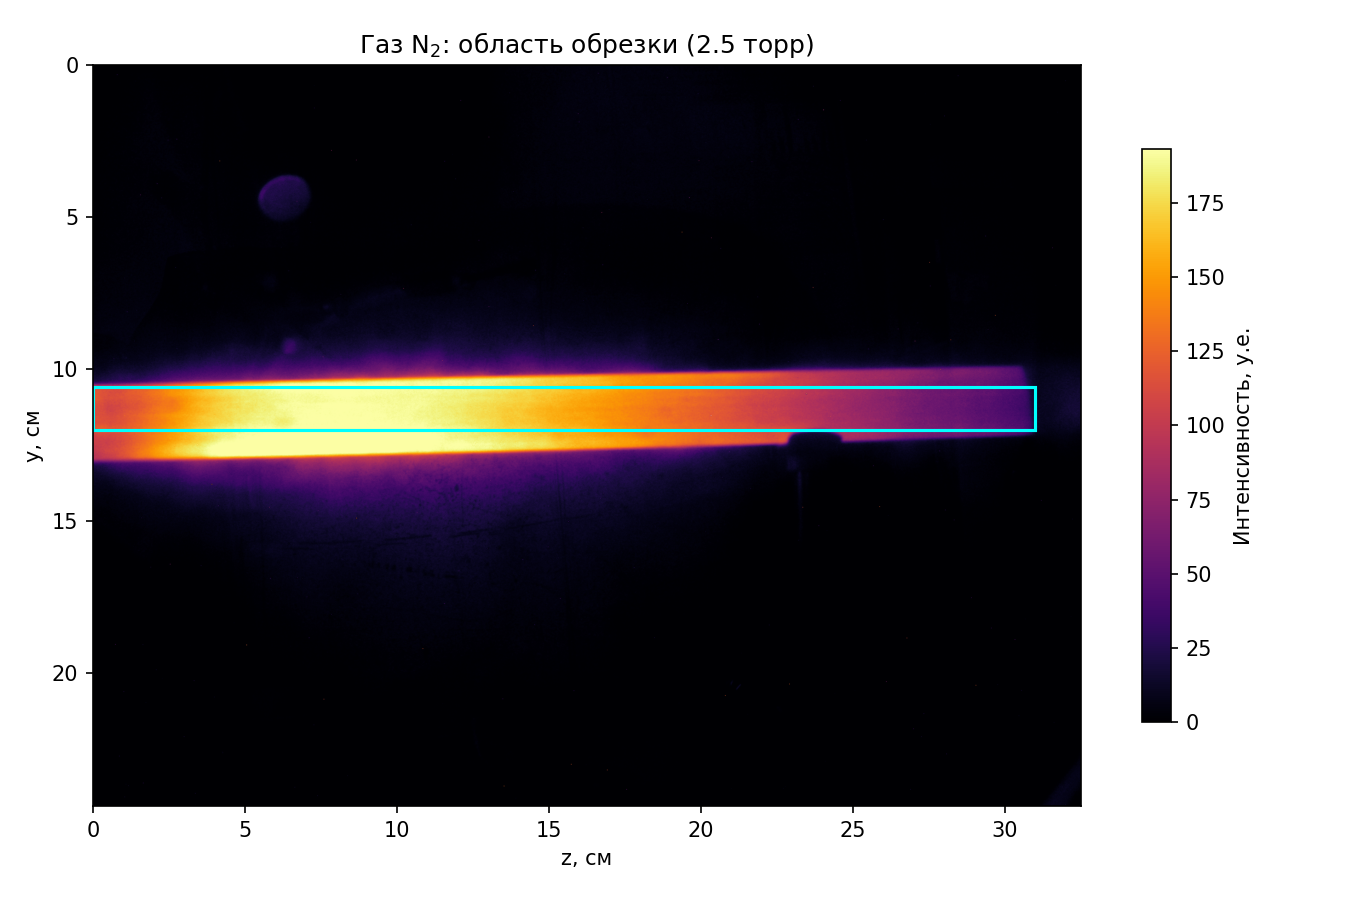
\includegraphics[width=\linewidth]{t1_crop_N2_2.5torr.png}
    \end{column}
    \begin{column}{0.43\textwidth}
      \small
      \begin{itemize}
        \item $B(z)$ --- средняя яркость полосы вдоль оси (143~px), фон вычтен
        \item масштаб по длине трубки: 0,0996~мм/px; проверка по диаметру --- 2\%
        \item \textbf{зелёный канал}: синий насыщен (до 58\% пикселей),
              красный слабый
        \item нужна только форма $B/B_\text{max}$; красный канал даёт те же
              $z_\text{max}$ в 5 режимах из 6
      \end{itemize}
    \end{column}
  \end{columns}
\end{frame}

\begin{frame}{Профили свечения $B(z)$}
  \centering
  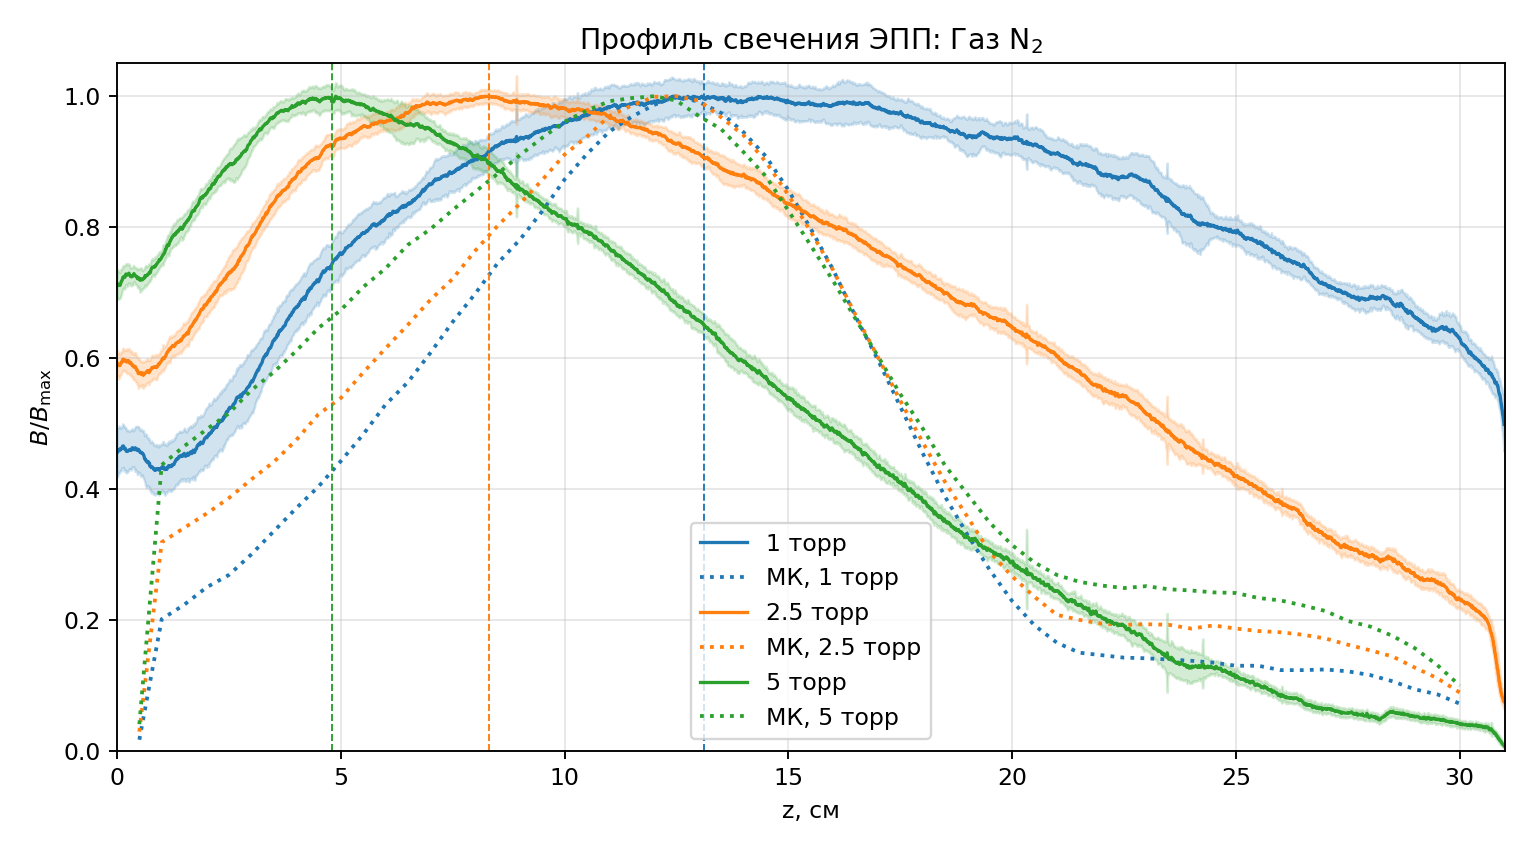
\includegraphics[width=0.49\linewidth]{t1_profile_N2.png}\hfill
  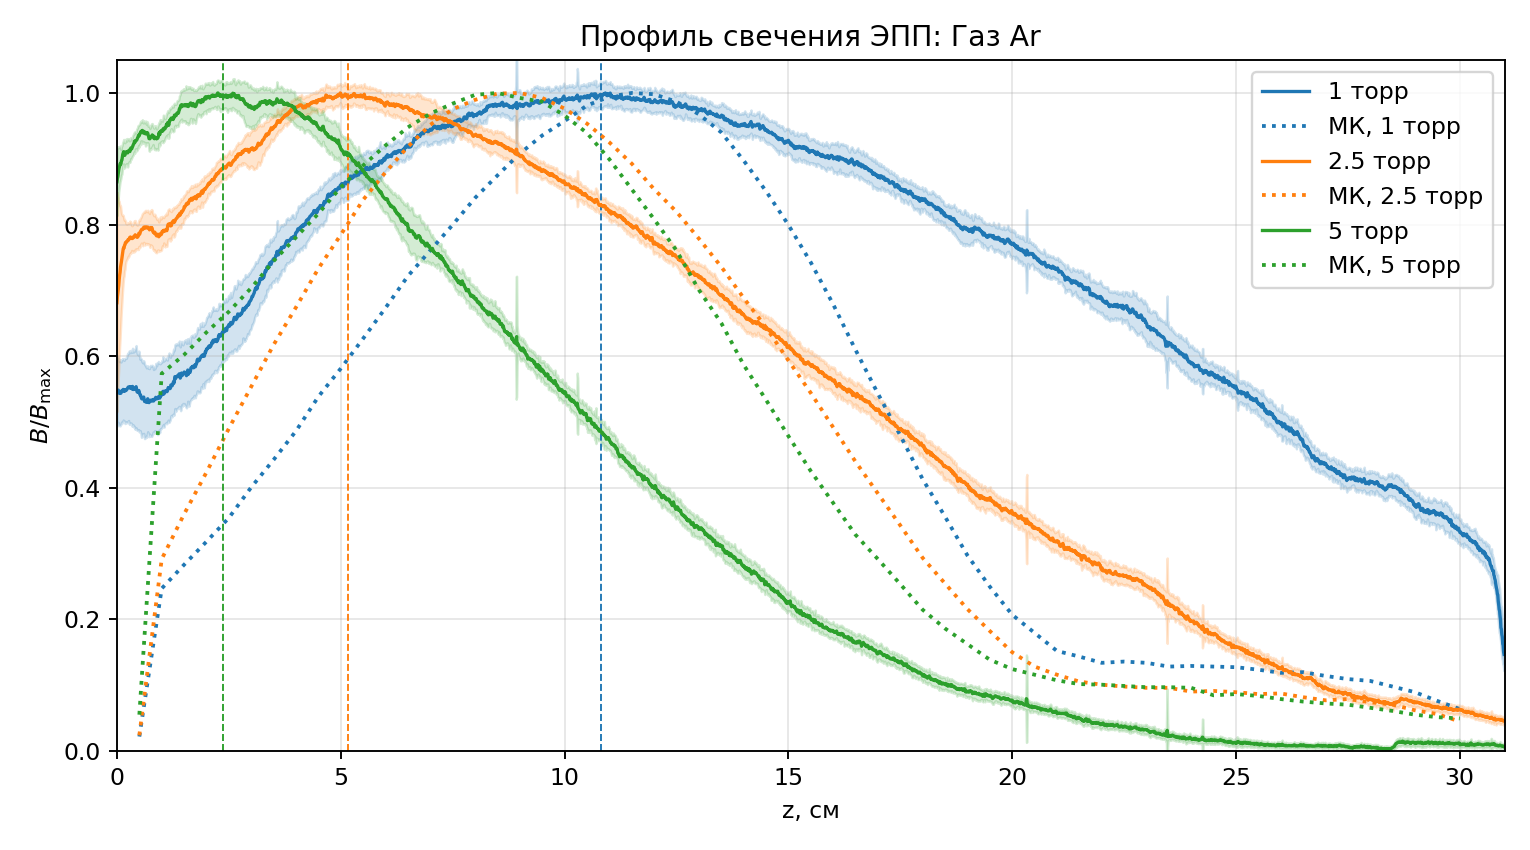
\includegraphics[width=0.49\linewidth]{t1_profile_Ar.png}

  \medskip
  \begin{itemize}
    \item максимум внутри трубки при всех давлениях
    \item с ростом $P_m$ максимум \textbf{сдвигается к выводному окну}, свечение у окна растёт
    \item пунктир --- расчёт Монте-Карло
  \end{itemize}
\end{frame}

\begin{frame}{Положение максимума}
  \begin{columns}[T]
    \begin{column}{0.48\textwidth}
      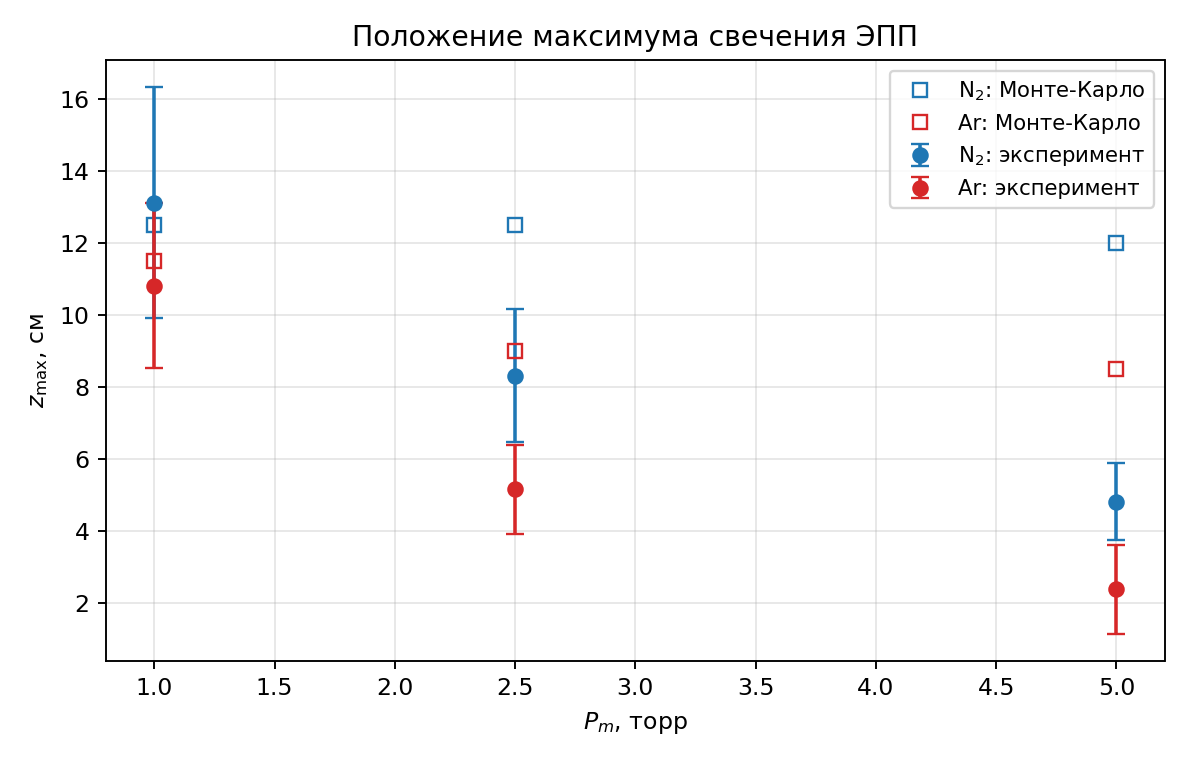
\includegraphics[width=\linewidth]{t1_zmax.png}
    \end{column}
    \begin{column}{0.5\textwidth}
      \small
      \begin{tabular}{lccc}
        \toprule
        & $P_m$, Торр & $z_\text{max}$, см & $z_R$, см \\
        \midrule
        $\Nt$ & 1   & $13{,}1\pm3{,}2$ & 9,4 \\
        $\Nt$ & 2,5 & $8{,}3\pm1{,}9$  & 6,9 \\
        $\Nt$ & 5   & $4{,}8\pm1{,}1$  & 5,5 \\
        \midrule
        Ar & 1   & $10{,}8\pm2{,}3$ & 6,5 \\
        Ar & 2,5 & $5{,}2\pm1{,}2$  & 4,8 \\
        Ar & 5   & $2{,}4\pm1{,}2$  & 3,8 \\
        \bottomrule
      \end{tabular}

      \medskip
      \begin{itemize}
        \item оценка $z_R$ даёт правильный порядок
        \item Ar/$\Nt$: опыт 0,82; 0,62; 0,50 --- оценка 0,69
        \item в опыте $z_\text{max} \propto P_m^{-0{,}6\ldots-0{,}9}$ ---
              сильнее, чем $P_m^{-1/3}$ (нагрев газа, отражение от стенки)
      \end{itemize}
    \end{column}
  \end{columns}
\end{frame}

\begin{frame}{Сравнение с расчётом Монте-Карло (программа «ДОЗА»)}
  \begin{columns}[T]
    \begin{column}{0.55\textwidth}
      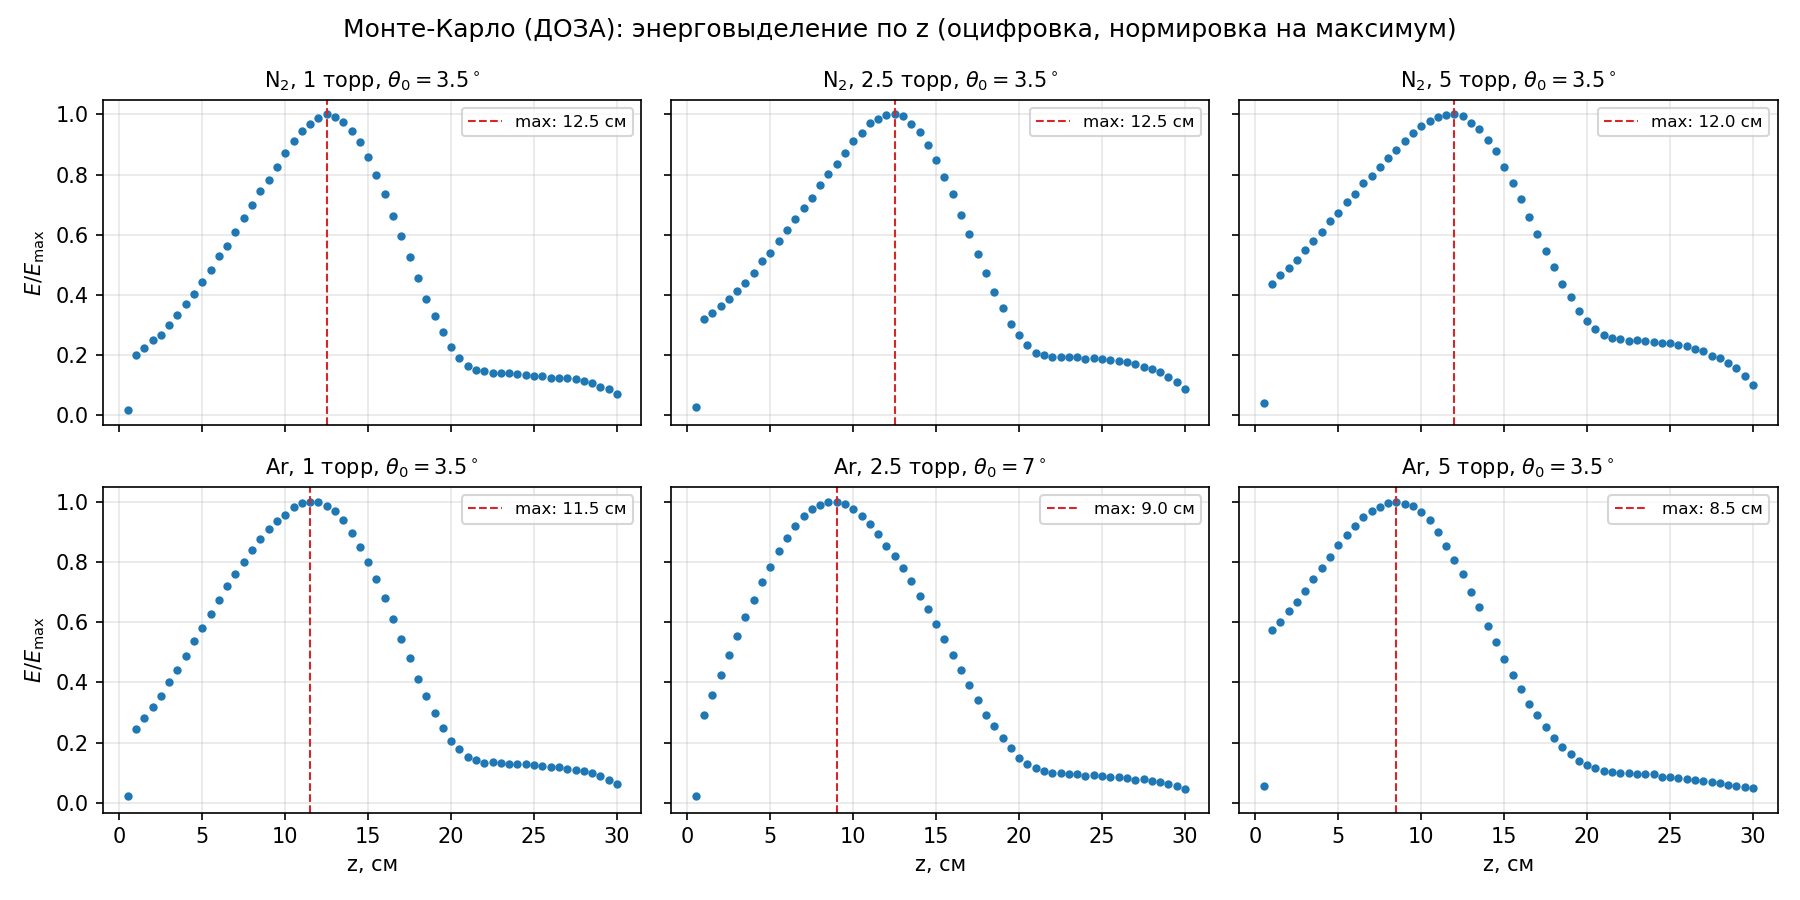
\includegraphics[width=\linewidth]{mc_digitized.png}
      {\scriptsize $E(z)/E_\text{max}$; сверху $\Nt$, снизу Ar; 1; 2,5; 5~Торр}
    \end{column}
    \begin{column}{0.43\textwidth}
      \small
      \textbf{Совпадает:}
      \begin{itemize}
        \item при 1~Торр: 12,5 и 11,5~см против $13{,}1$ и $10{,}8$~см
        \item в Ar максимум ближе к окну, чем в $\Nt$
      \end{itemize}
      \textbf{Не совпадает:}
      \begin{itemize}
        \item в $\Nt$ расчётный максимум почти не сдвигается (12,5 $\to$ 12,0~см)
        \item площадь под $E(z)$ почти не растёт с давлением, хотя
              должна расти $\propto P_m$
      \end{itemize}
      $\Rightarrow$ давление в расчёте, вероятно, задано не так, как в опыте
    \end{column}
  \end{columns}
\end{frame}

\begin{frame}{Сравнение с пособием (рис.~6.8)}
  \begin{columns}[c]
    \begin{column}{0.4\textwidth}
      \centering
      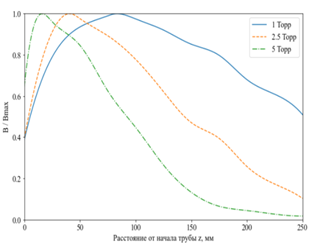
\includegraphics[width=\linewidth]{book_fig6_8_Ar.png}\\
      {\scriptsize Ar, трубка $\varnothing 20$~мм, 1; 2,5; 5~Торр}
    \end{column}
    \begin{column}{0.56\textwidth}
      \begin{tabular}{lccc}
        \toprule
        Ar, Торр & 1 & 2,5 & 5 \\
        \midrule
        пособие, см & 8,5 & 4,0 & 1,5 \\
        наш опыт, см & 10,8 & 5,2 & 2,4 \\
        \bottomrule
      \end{tabular}

      \medskip
      \begin{itemize}
        \item та же форма и тот же сдвиг максимума
        \item тот же уровень свечения у начала трубки:
              $\approx 0{,}45$--$0{,}55\,B_\text{max}$ при 1~Торр
        \item наши максимумы дальше: диаметр трубки объясняет
              лишь 10--15\% ($z_R \propto R^{2/3}$)
      \end{itemize}
    \end{column}
  \end{columns}
\end{frame}

% ===============================================================
\section{ВЧ-ёмкостный разряд}
% ===============================================================

\begin{frame}{ВЧЕ-разряд: установка и формы разряда}
  \begin{columns}[T]
    \begin{column}{0.5\textwidth}
      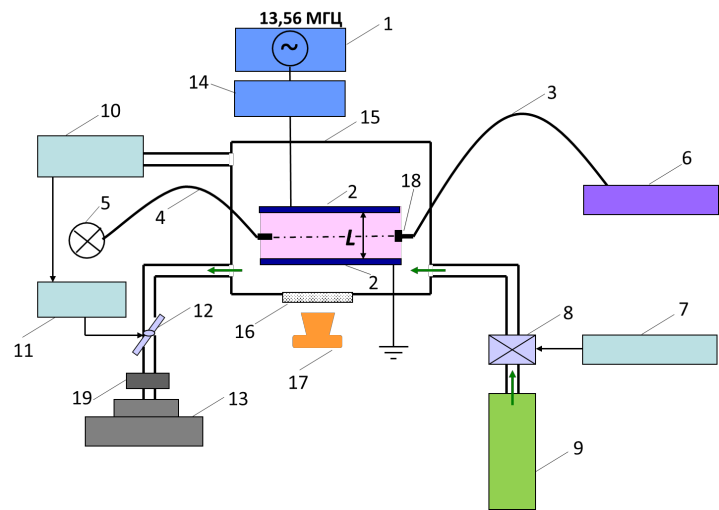
\includegraphics[width=\linewidth]{scheme_rf.png}
      {\small $f = 13{,}56$~МГц, 50~Вт, зазор $L = 37{,}2\pm0{,}2$~мм}
    \end{column}
    \begin{column}{0.48\textwidth}
      \small
      \textbf{$\alpha$-форма} (слаботочная): объёмная ионизация электронами,
      нагретыми ВЧ-полем; свечение широкое, у электродов тёмные слои.

      \medskip
      \textbf{$\gamma$-форма} (сильноточная): вторичная эмиссия из
      электродов, лавина в слоях; яркие тонкие слои у электродов,
      тёмные промежутки и светящаяся зона в центре.

      \medskip
      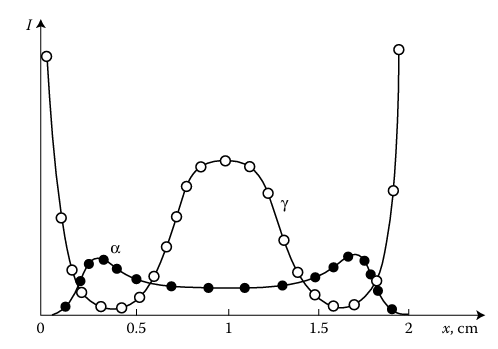
\includegraphics[width=0.75\linewidth]{rf_profile_alpha_gamma.png}
    \end{column}
  \end{columns}
\end{frame}

\begin{frame}{Профили свечения $I(L)$}
  \centering
  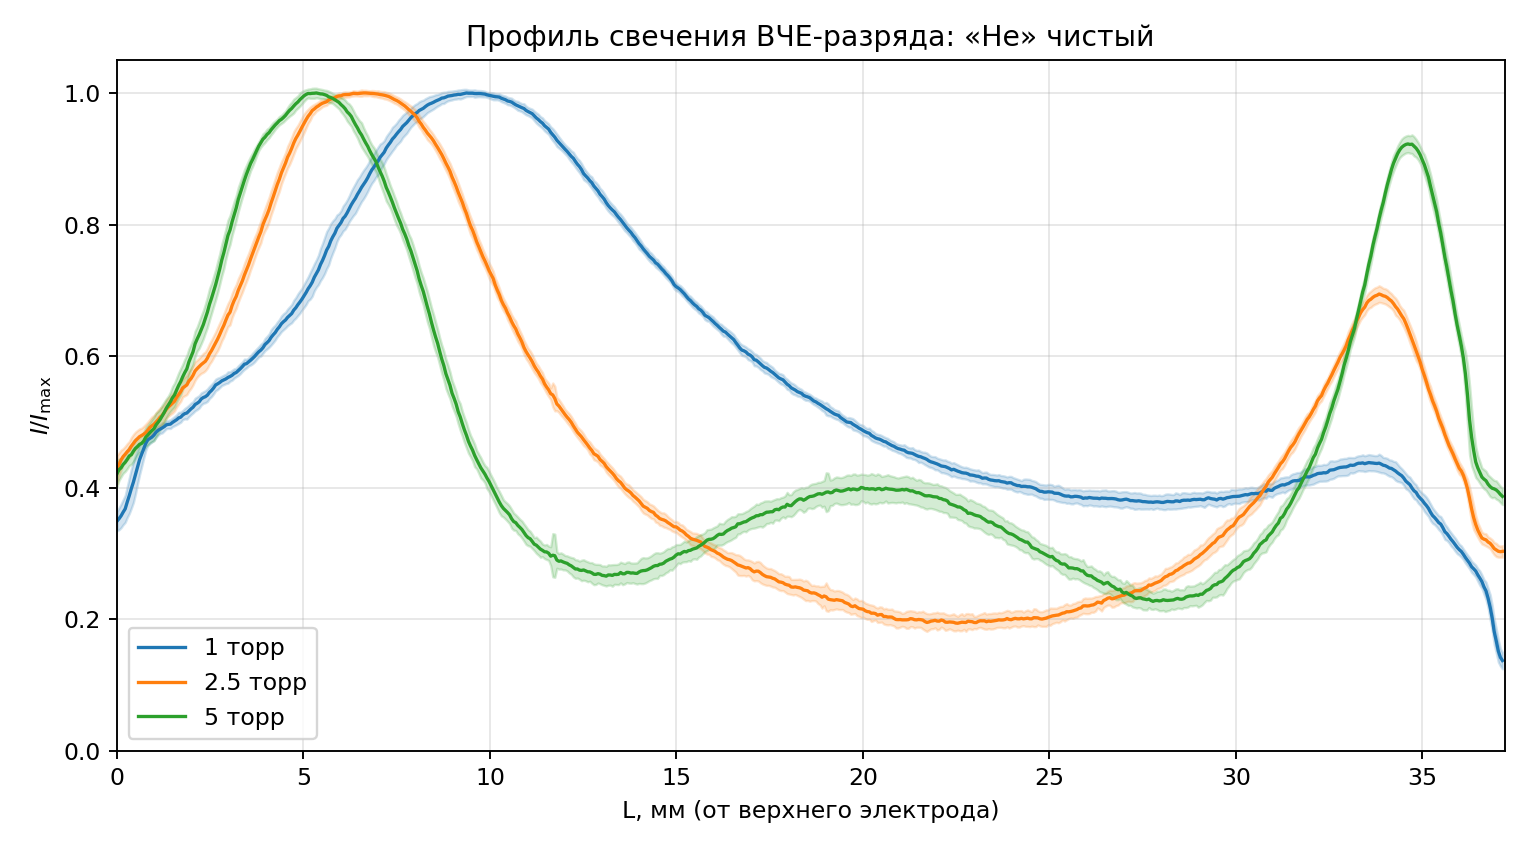
\includegraphics[width=0.49\linewidth]{t2_profile_He.png}\hfill
  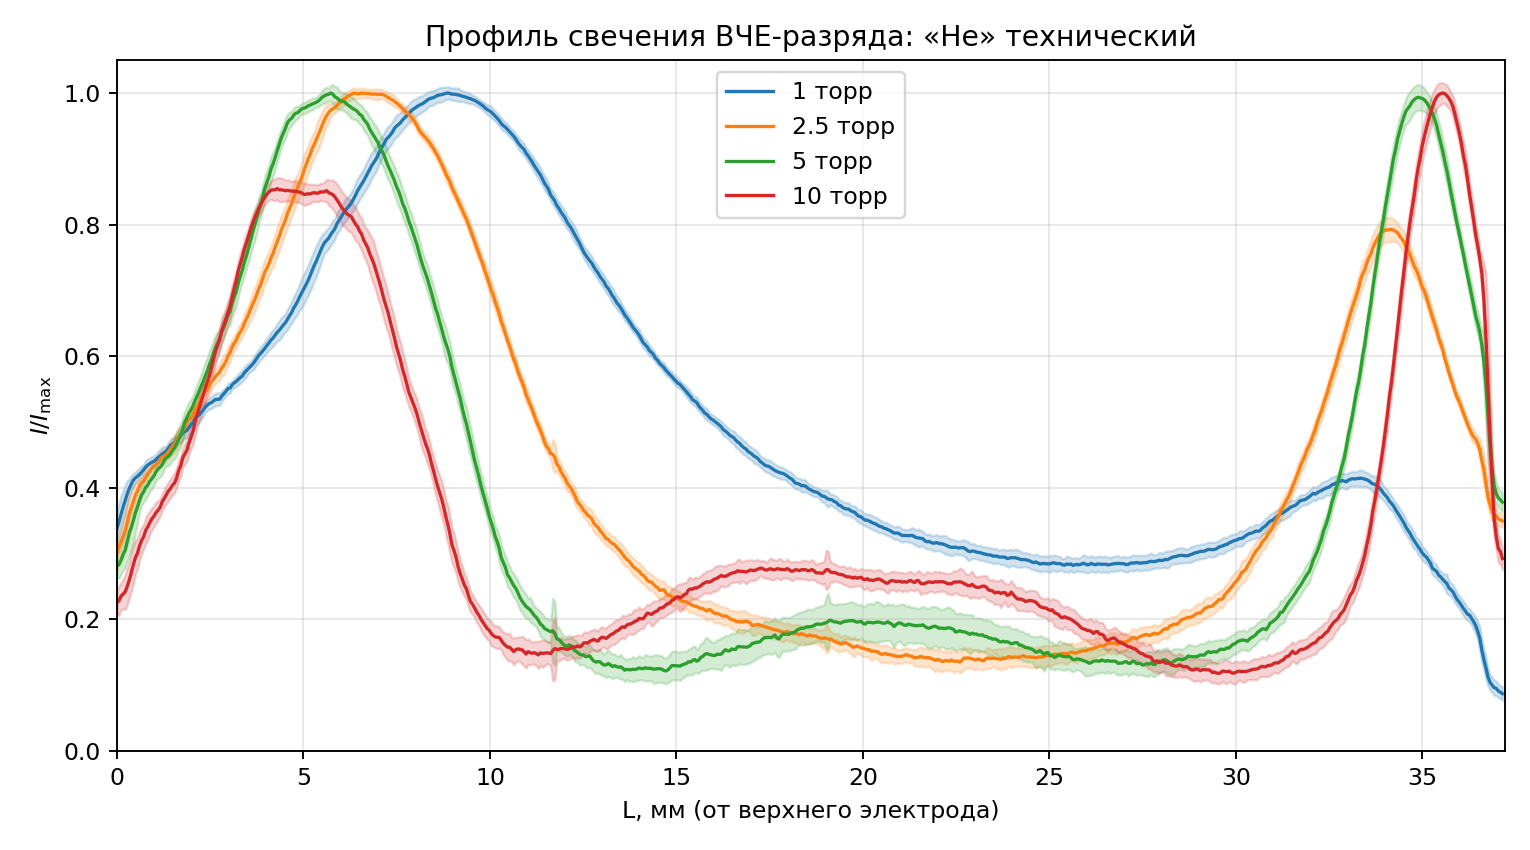
\includegraphics[width=0.49\linewidth]{t2_profile_He_tech.png}

  {\small слева чистый He, справа технический}
  \begin{itemize}
    \item 1~Торр: свечение по всему промежутку --- $\alpha$-форма
    \item с ростом $P_m$ светящиеся слои поджимаются к электродам (9,5 $\to$ 1,7--5~мм)
    \item 5~Торр: яркие слои, тёмные промежутки, зона в центре --- $\gamma$-форма
  \end{itemize}
\end{frame}

\begin{frame}{Переход $\alpha\to\gamma$}
  \begin{columns}[T]
    \begin{column}{0.4\textwidth}
      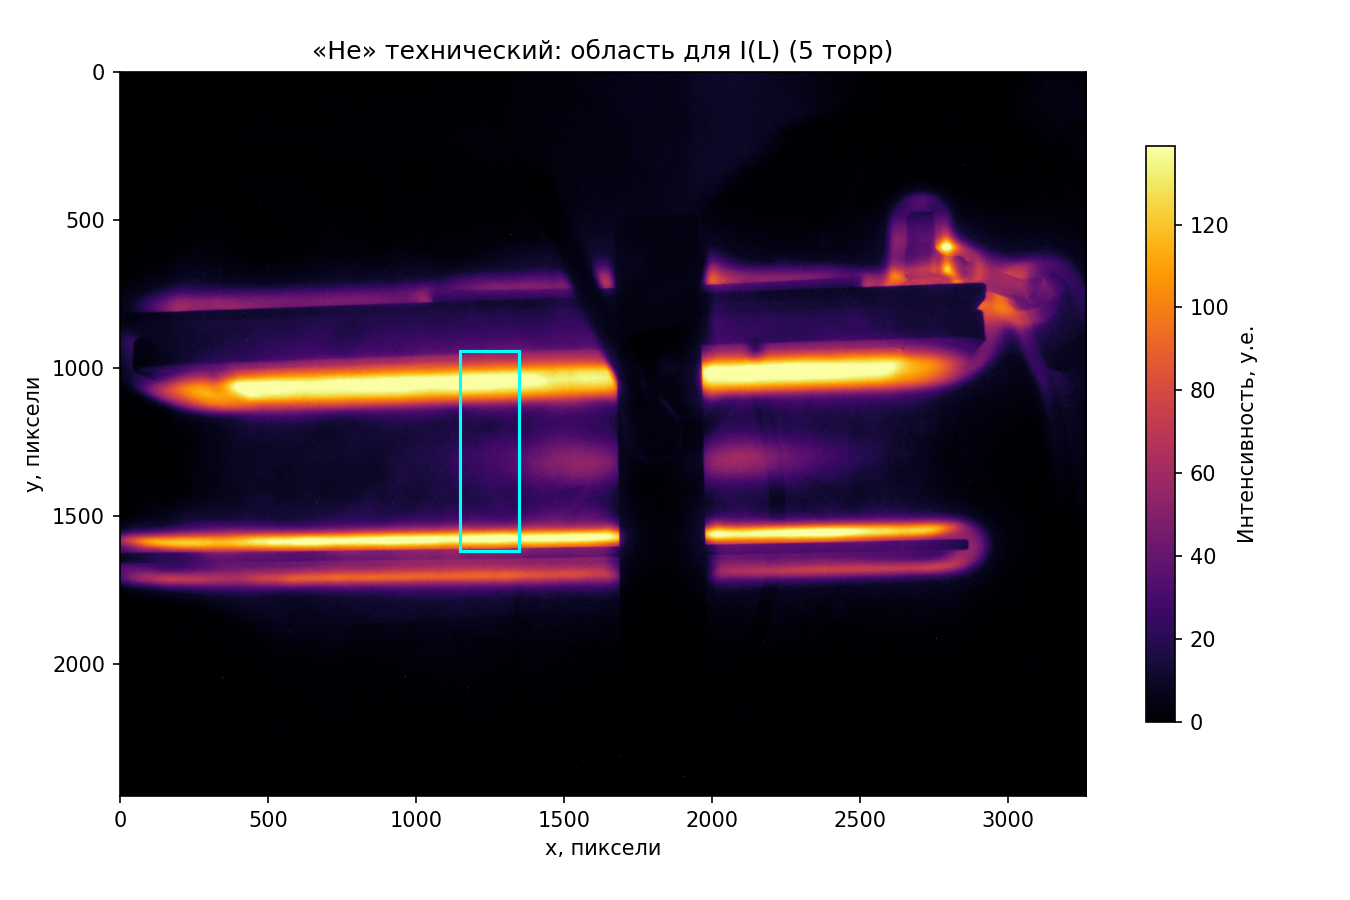
\includegraphics[width=\linewidth]{t2_crop_He_tech_5torr.png}
      {\scriptsize технический He, 5~Торр}
    \end{column}
    \begin{column}{0.58\textwidth}
      Признак перехода --- появление центральной страты:
      \[
        (P_m L)_\text{He} = 14{,}5\pm0{,}4,\quad
        (P_m L)_\text{He техн} = 13{,}0\pm0{,}4~\text{Торр}\cdot\text{см}
      \]
      \begin{itemize}
        \item \textbf{рис.~4 методички} (технический He, 30~мм, 50~Вт):
              $\gamma$-форма уже при 15~Торр$\cdot$см --- \alert{согласуется}
        \item \textbf{рис.~6} (граница для чистого He $\approx 160$):
              у нас на порядок ниже --- примеси, материал электродов,
              мощность
        \item в техническом He переход раньше (3,5 против 3,9~Торр)
      \end{itemize}
    \end{column}
  \end{columns}
\end{frame}

\begin{frame}{Спектры: что светится}
  \begin{columns}[T]
    \begin{column}{0.5\textwidth}
      \centering
      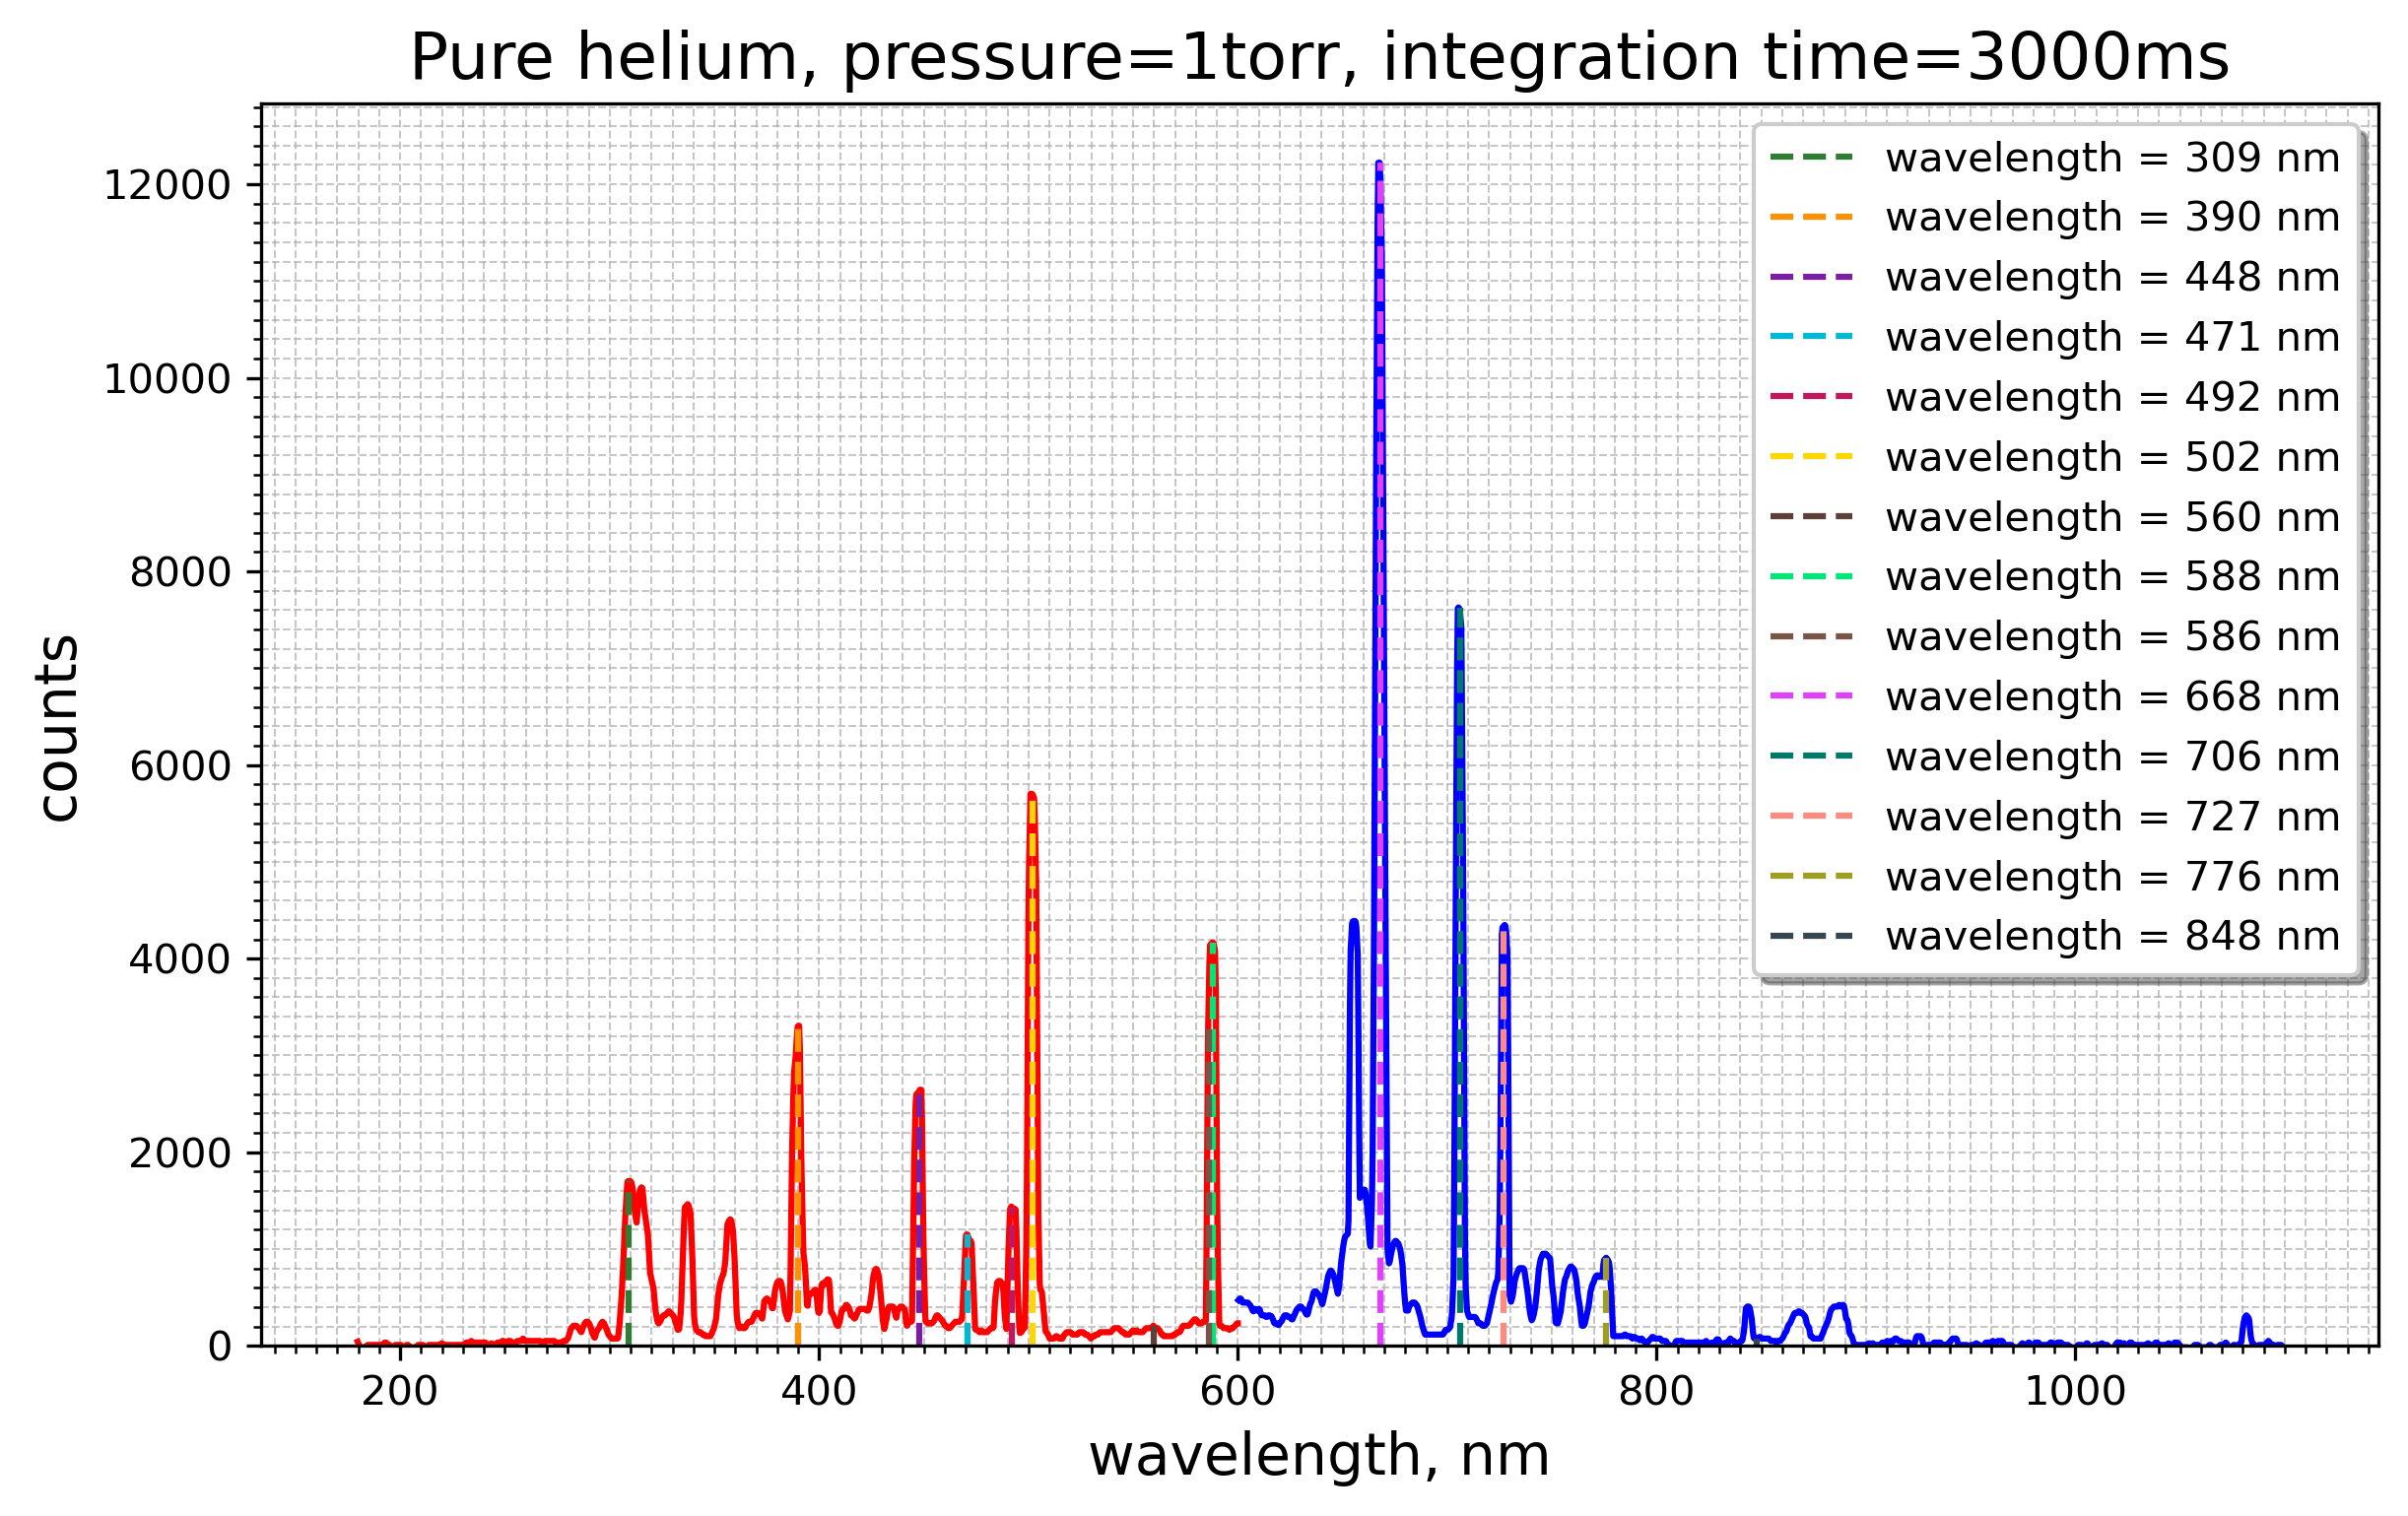
\includegraphics[height=0.38\textheight]{spec_He_1torr.png}\\
      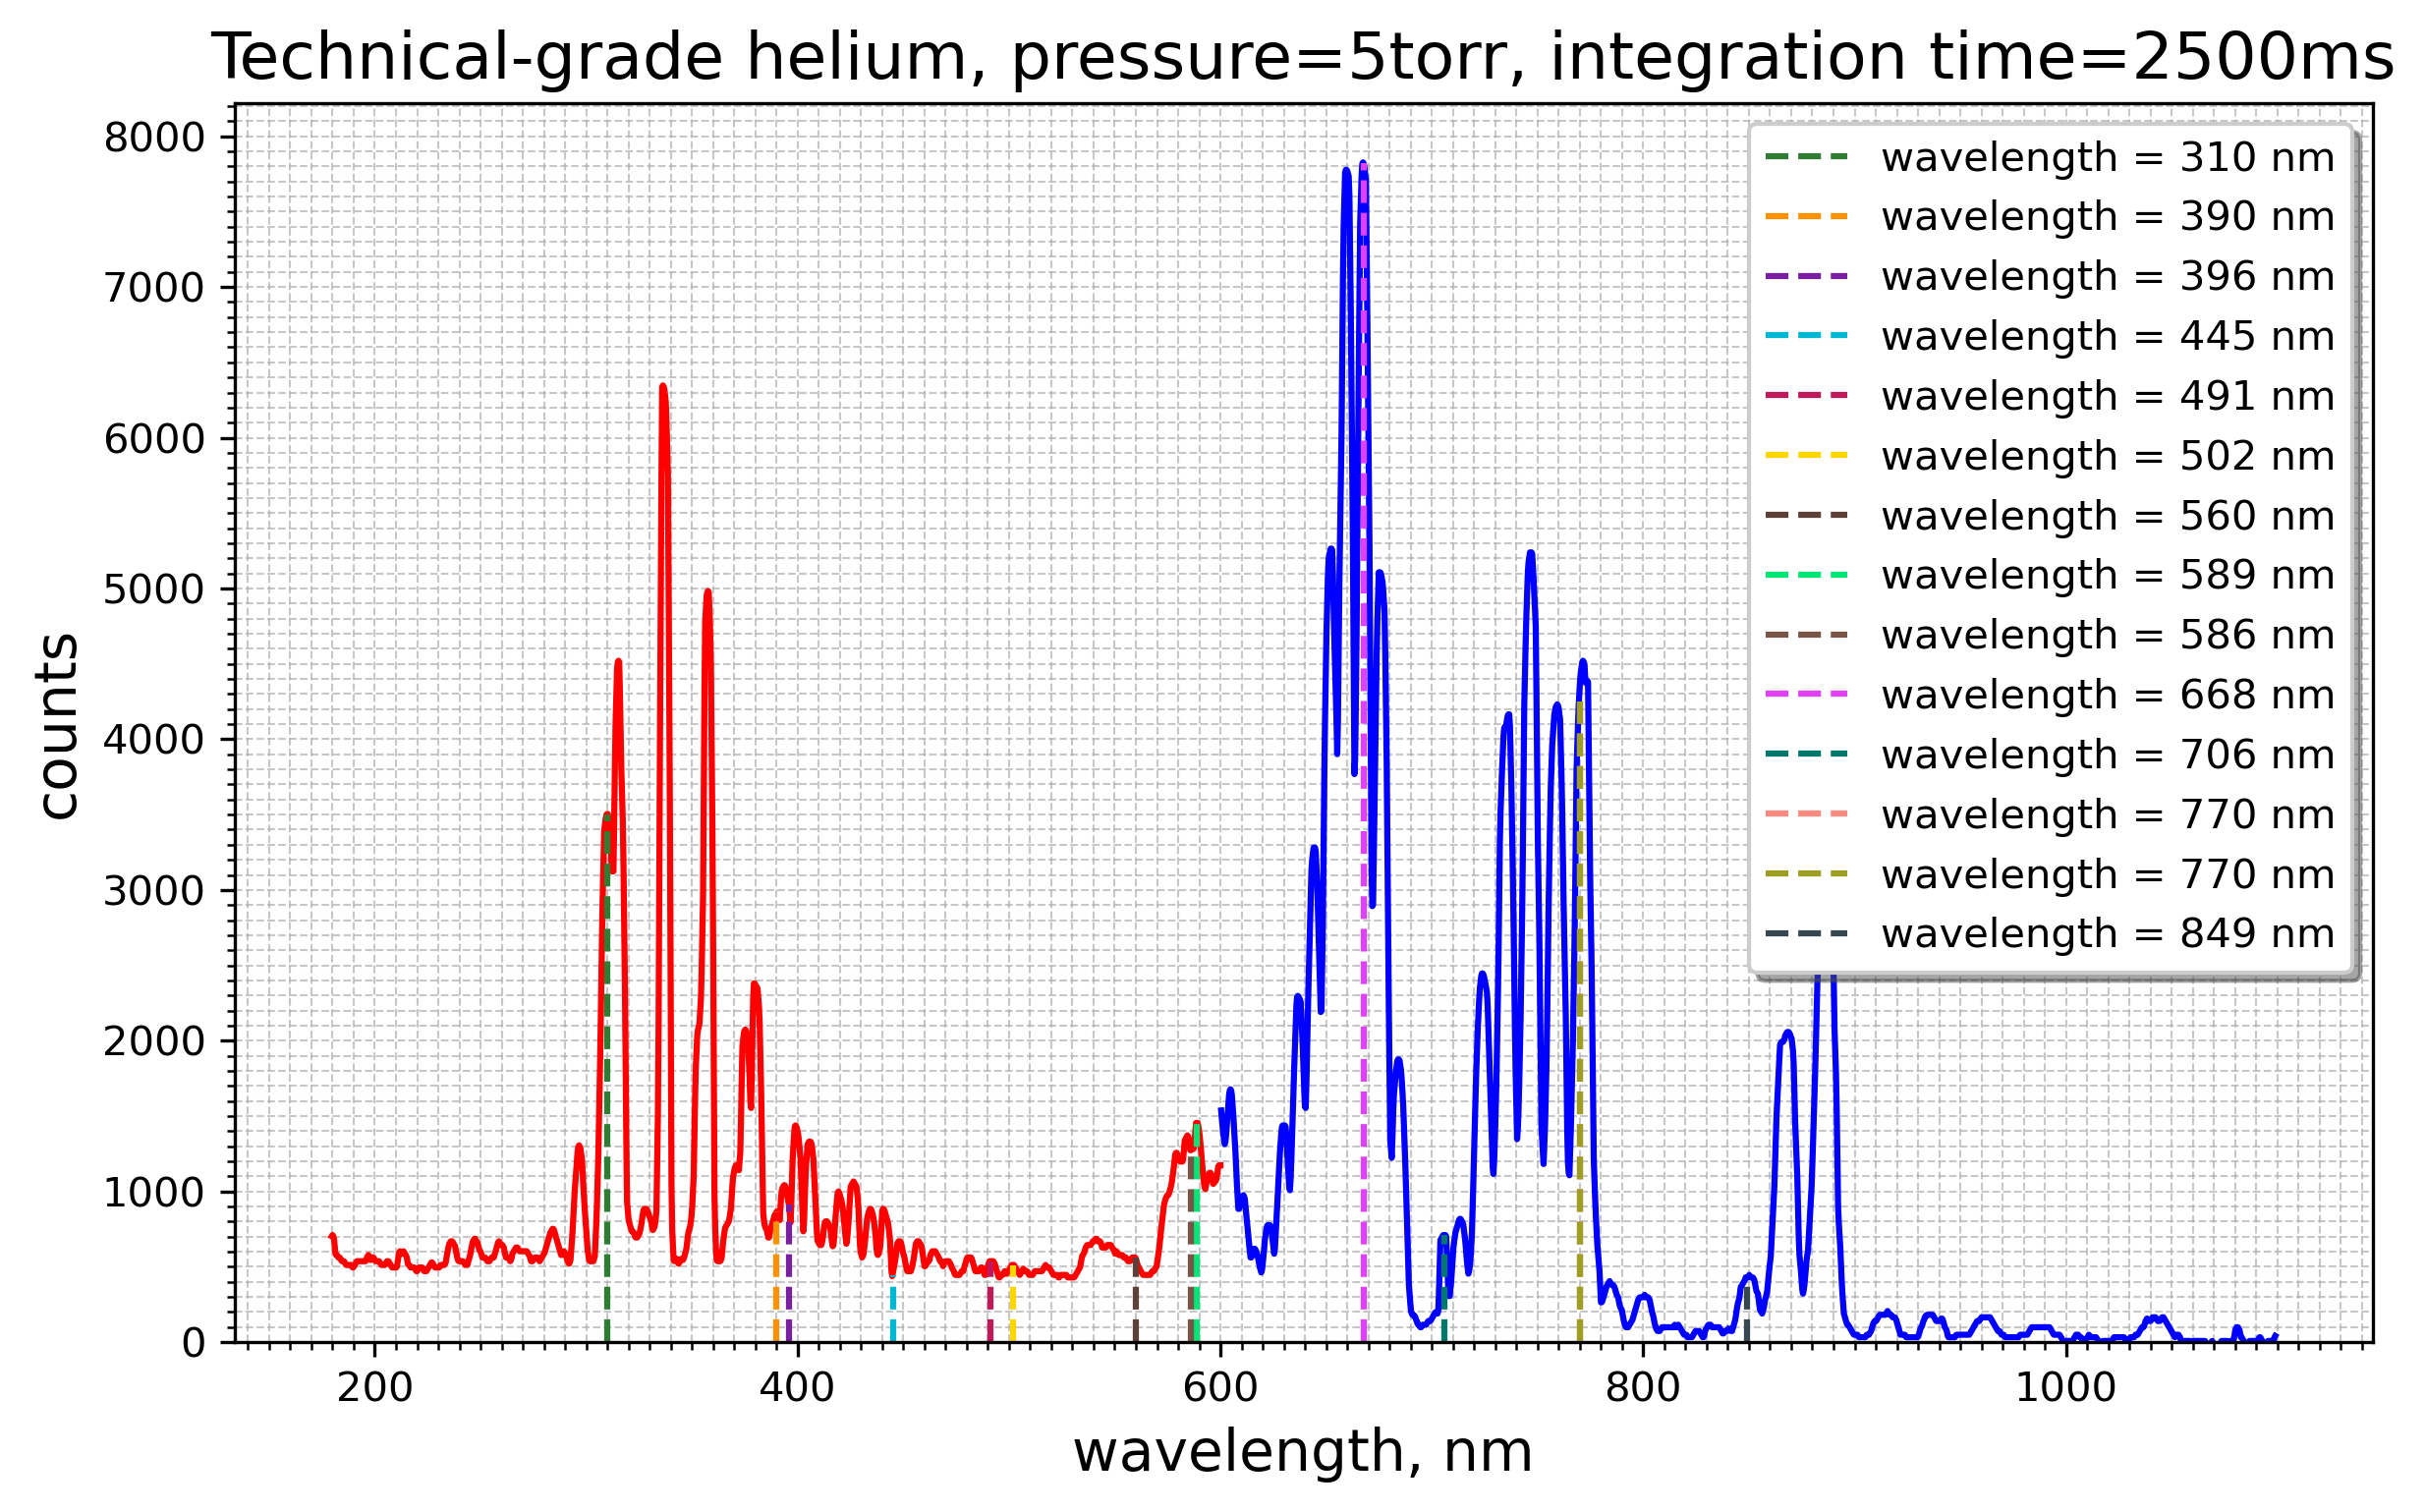
\includegraphics[height=0.38\textheight]{spec_He_tech_5torr.png}
    \end{column}
    \begin{column}{0.48\textwidth}
      \small
      \begin{tabular}{ll}
        \toprule
        $\lambda$, нм & источник \\
        \midrule
        308--310 & OH (пары воды) \\
        315, 337, 357, 380 & $\Nt$ (УФ) \\
        391, 428 & $\mathrm{N_2^+}$ \\
        580--780 & $\Nt$ (красные полосы) \\
        447, 502, 588, 668, 706 & He \\
        \bottomrule
      \end{tabular}

      \medskip
      \begin{itemize}
        \item сверху: чистый He, 1~Торр --- линии гелия
        \item снизу: технический He, 5~Торр --- полосы азота
        \item две линейки спектрометра имеют разную чувствительность
              $\Rightarrow$ сравниваем пики одной линейки
      \end{itemize}
    \end{column}
  \end{columns}
\end{frame}

\begin{frame}{Когда азот перерастает гелий; доля примеси}
  \begin{columns}[T]
    \begin{column}{0.48\textwidth}
      \small
      Пики 337~нм ($\Nt$) и 502~нм (He), линейка Master:
      \begin{tabular}{lccc}
        \toprule
        $P_m$, Торр & 1 & 2,5 & 5 \\
        \midrule
        He чистый & 0,25 & 0,23 & $\approx 11$ \\
        He техн.  & 0,64 & 1,2 & $\gtrsim 13$ \\
        \bottomrule
      \end{tabular}

      \medskip
      \begin{itemize}
        \item технический He: азот сравним с гелием уже при 2,5~Торр
        \item в обоих газах между 2,5 и 5~Торр азот преобладает
      \end{itemize}
    \end{column}
    \begin{column}{0.5\textwidth}
      \small
      Азот перехватывает возбуждение, если $\tau_\text{пер} = 1/(kN_{\Nt})$
      меньше времени высвечивания He $\tau \sim 1$~мкс:
      \[
        N_{\Nt}^* = \frac{1}{k\tau} \approx 10^{15}~\text{см}^{-3},\qquad
        x_{\Nt} = \frac{N_{\Nt}^*}{P^*/kT} \approx \frac{3{,}1\%}{P^*[\text{Торр}]}
      \]
      $\Rightarrow$ \textbf{$x_{\Nt} \sim 1\%$} (0,6--1,2\%)

      \medskip
      \alert{Оговорка:} в том же интервале давлений разряд переходит в
      $\gamma$-форму, это тоже может усиливать полосы азота.
    \end{column}
  \end{columns}
\end{frame}

\begin{frame}{Красный канал камеры}
  \centering
  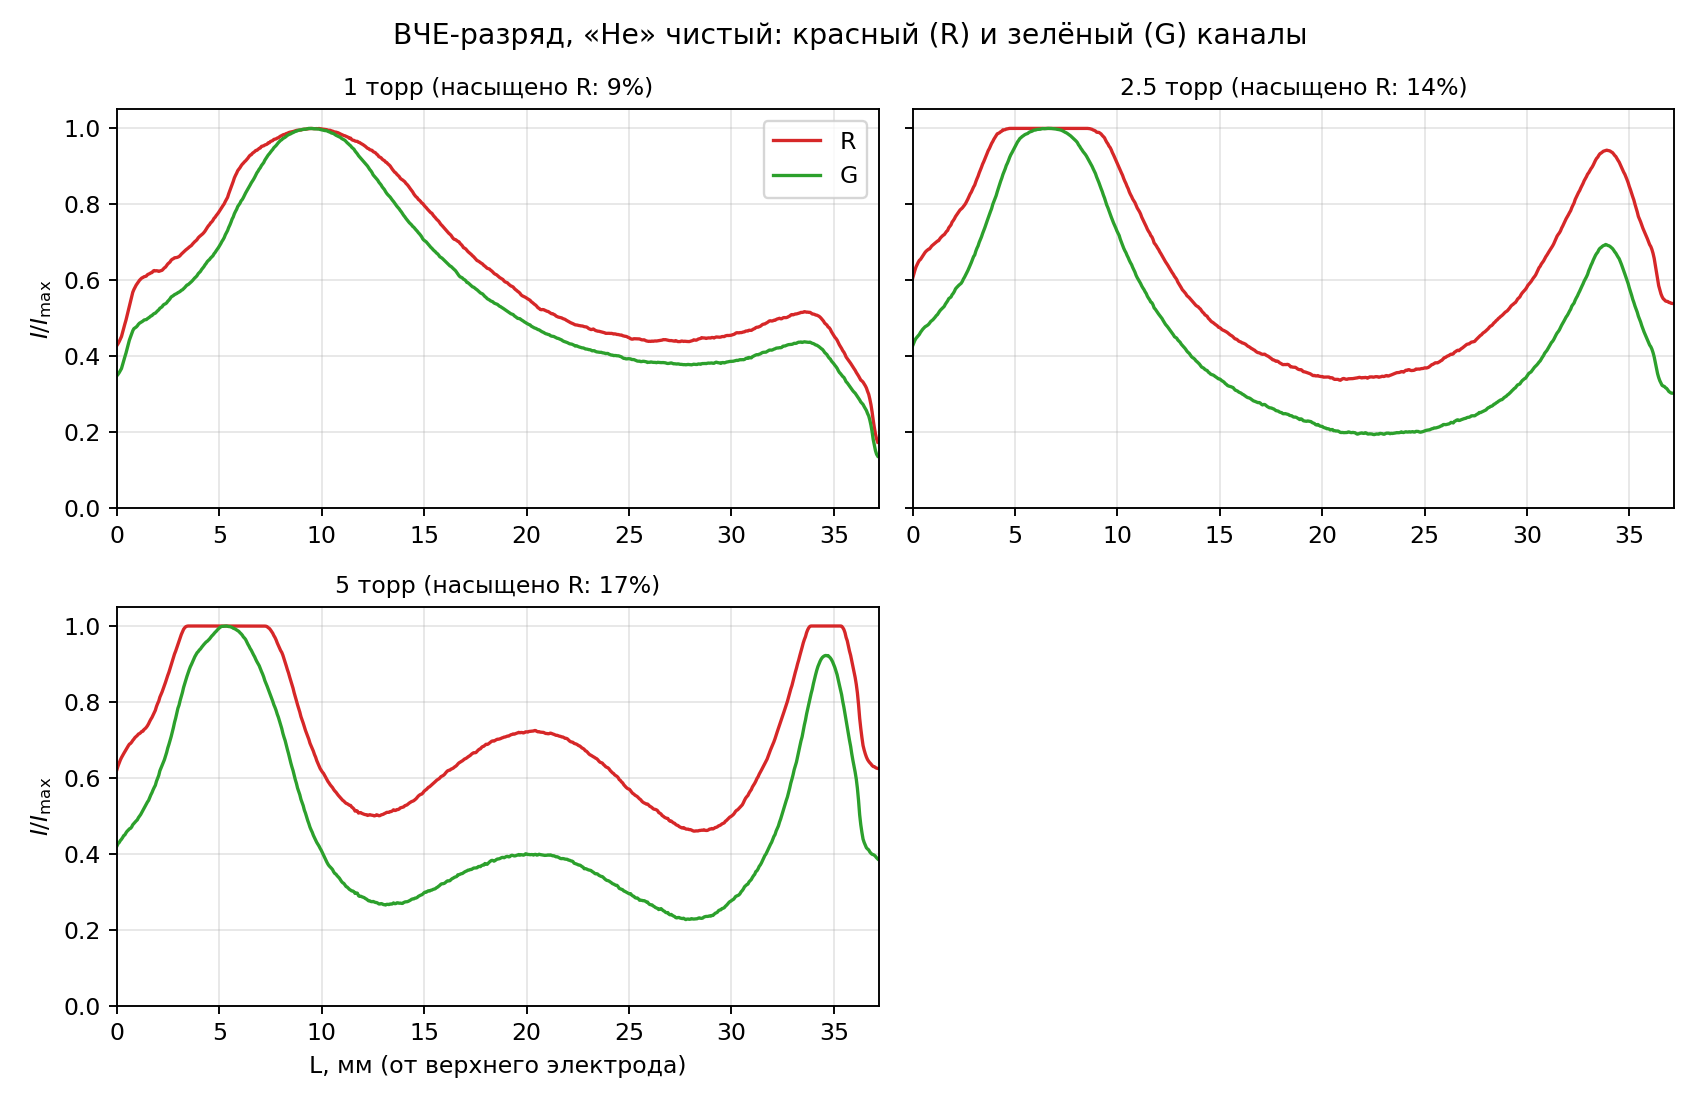
\includegraphics[width=0.49\linewidth]{t2_profile_red_He.png}\hfill
  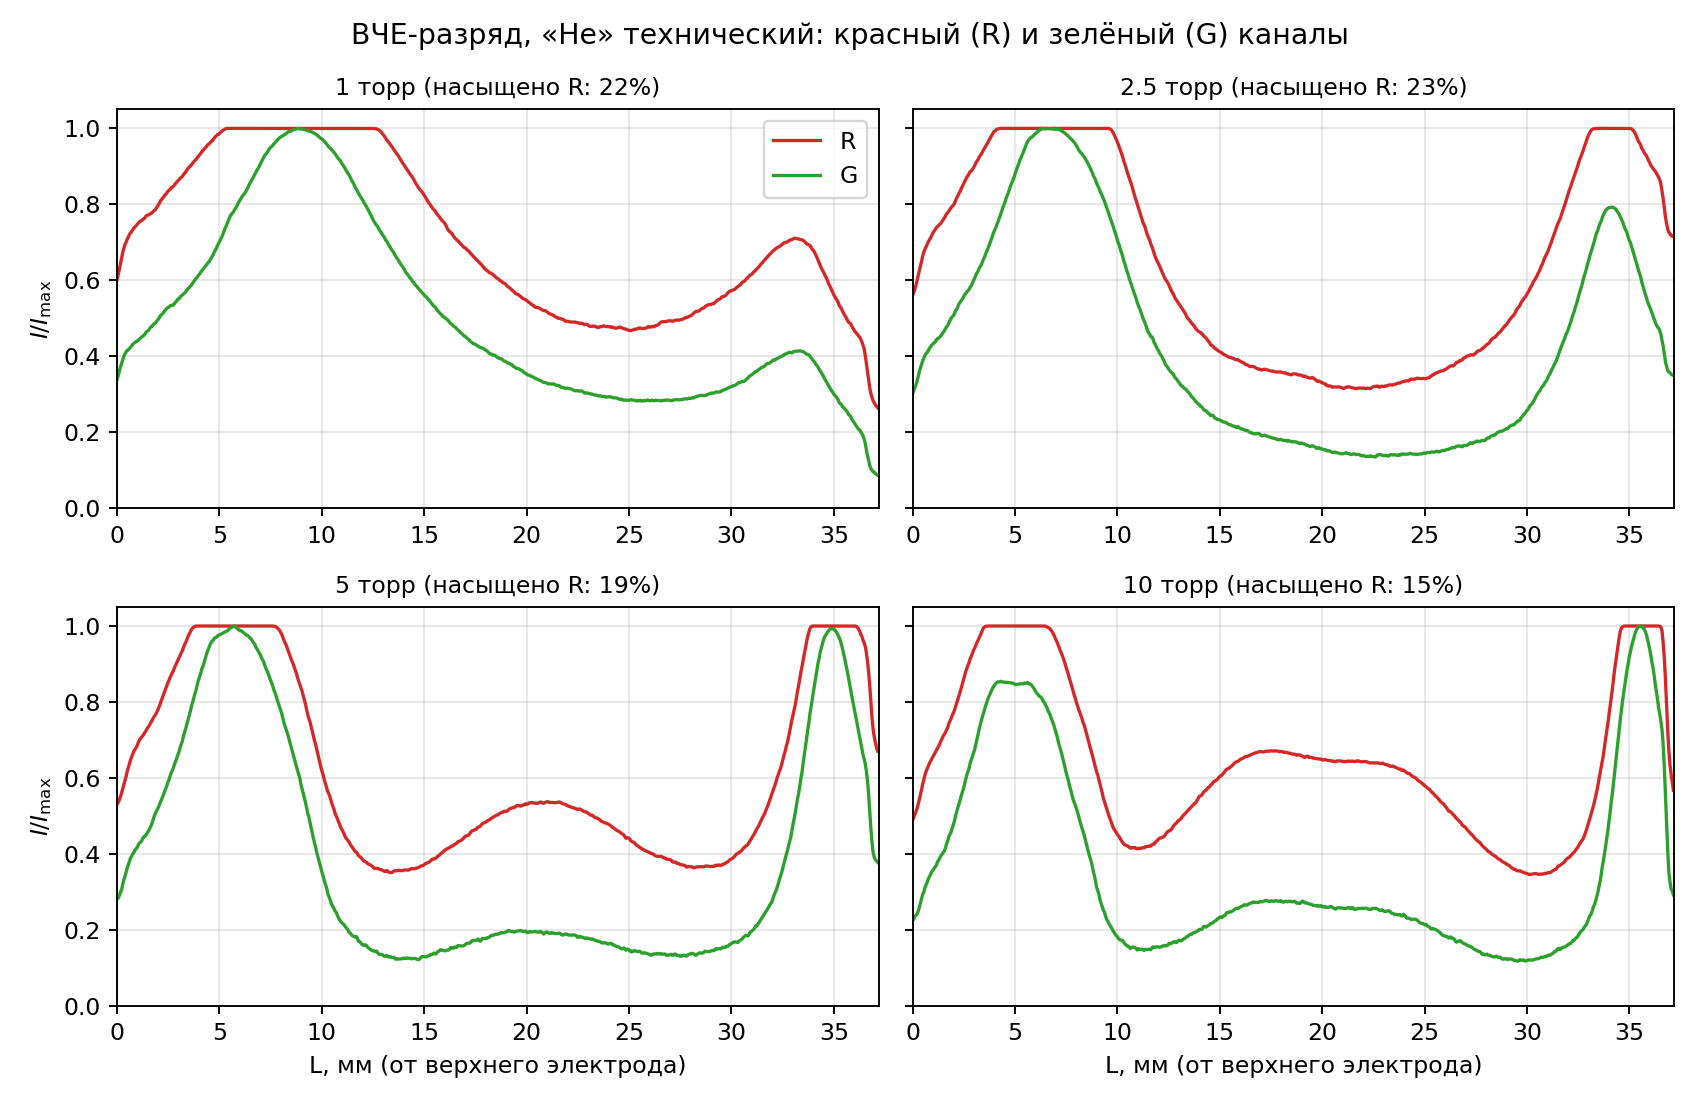
\includegraphics[width=0.49\linewidth]{t2_profile_red_He_tech.png}

  {\small слева чистый He, справа технический; R и G нормированы каждый на свой максимум}
  \begin{itemize}
    \item в красный канал попадают и полосы $\Nt$, и линии He 668, 706, 728~нм
    \item центр в R ярче, чем в G, там, где по спектрам много азота
          (в том числе чистый He при 5~Торр); при 1~Торр в чистом He каналы совпадают
    \item красный канал частично насыщен $\Rightarrow$ только качественное подтверждение
  \end{itemize}
\end{frame}

\begin{frame}{Оптическая прозрачность плазмы}
  \begin{columns}[T]
    \begin{column}{0.58\textwidth}
      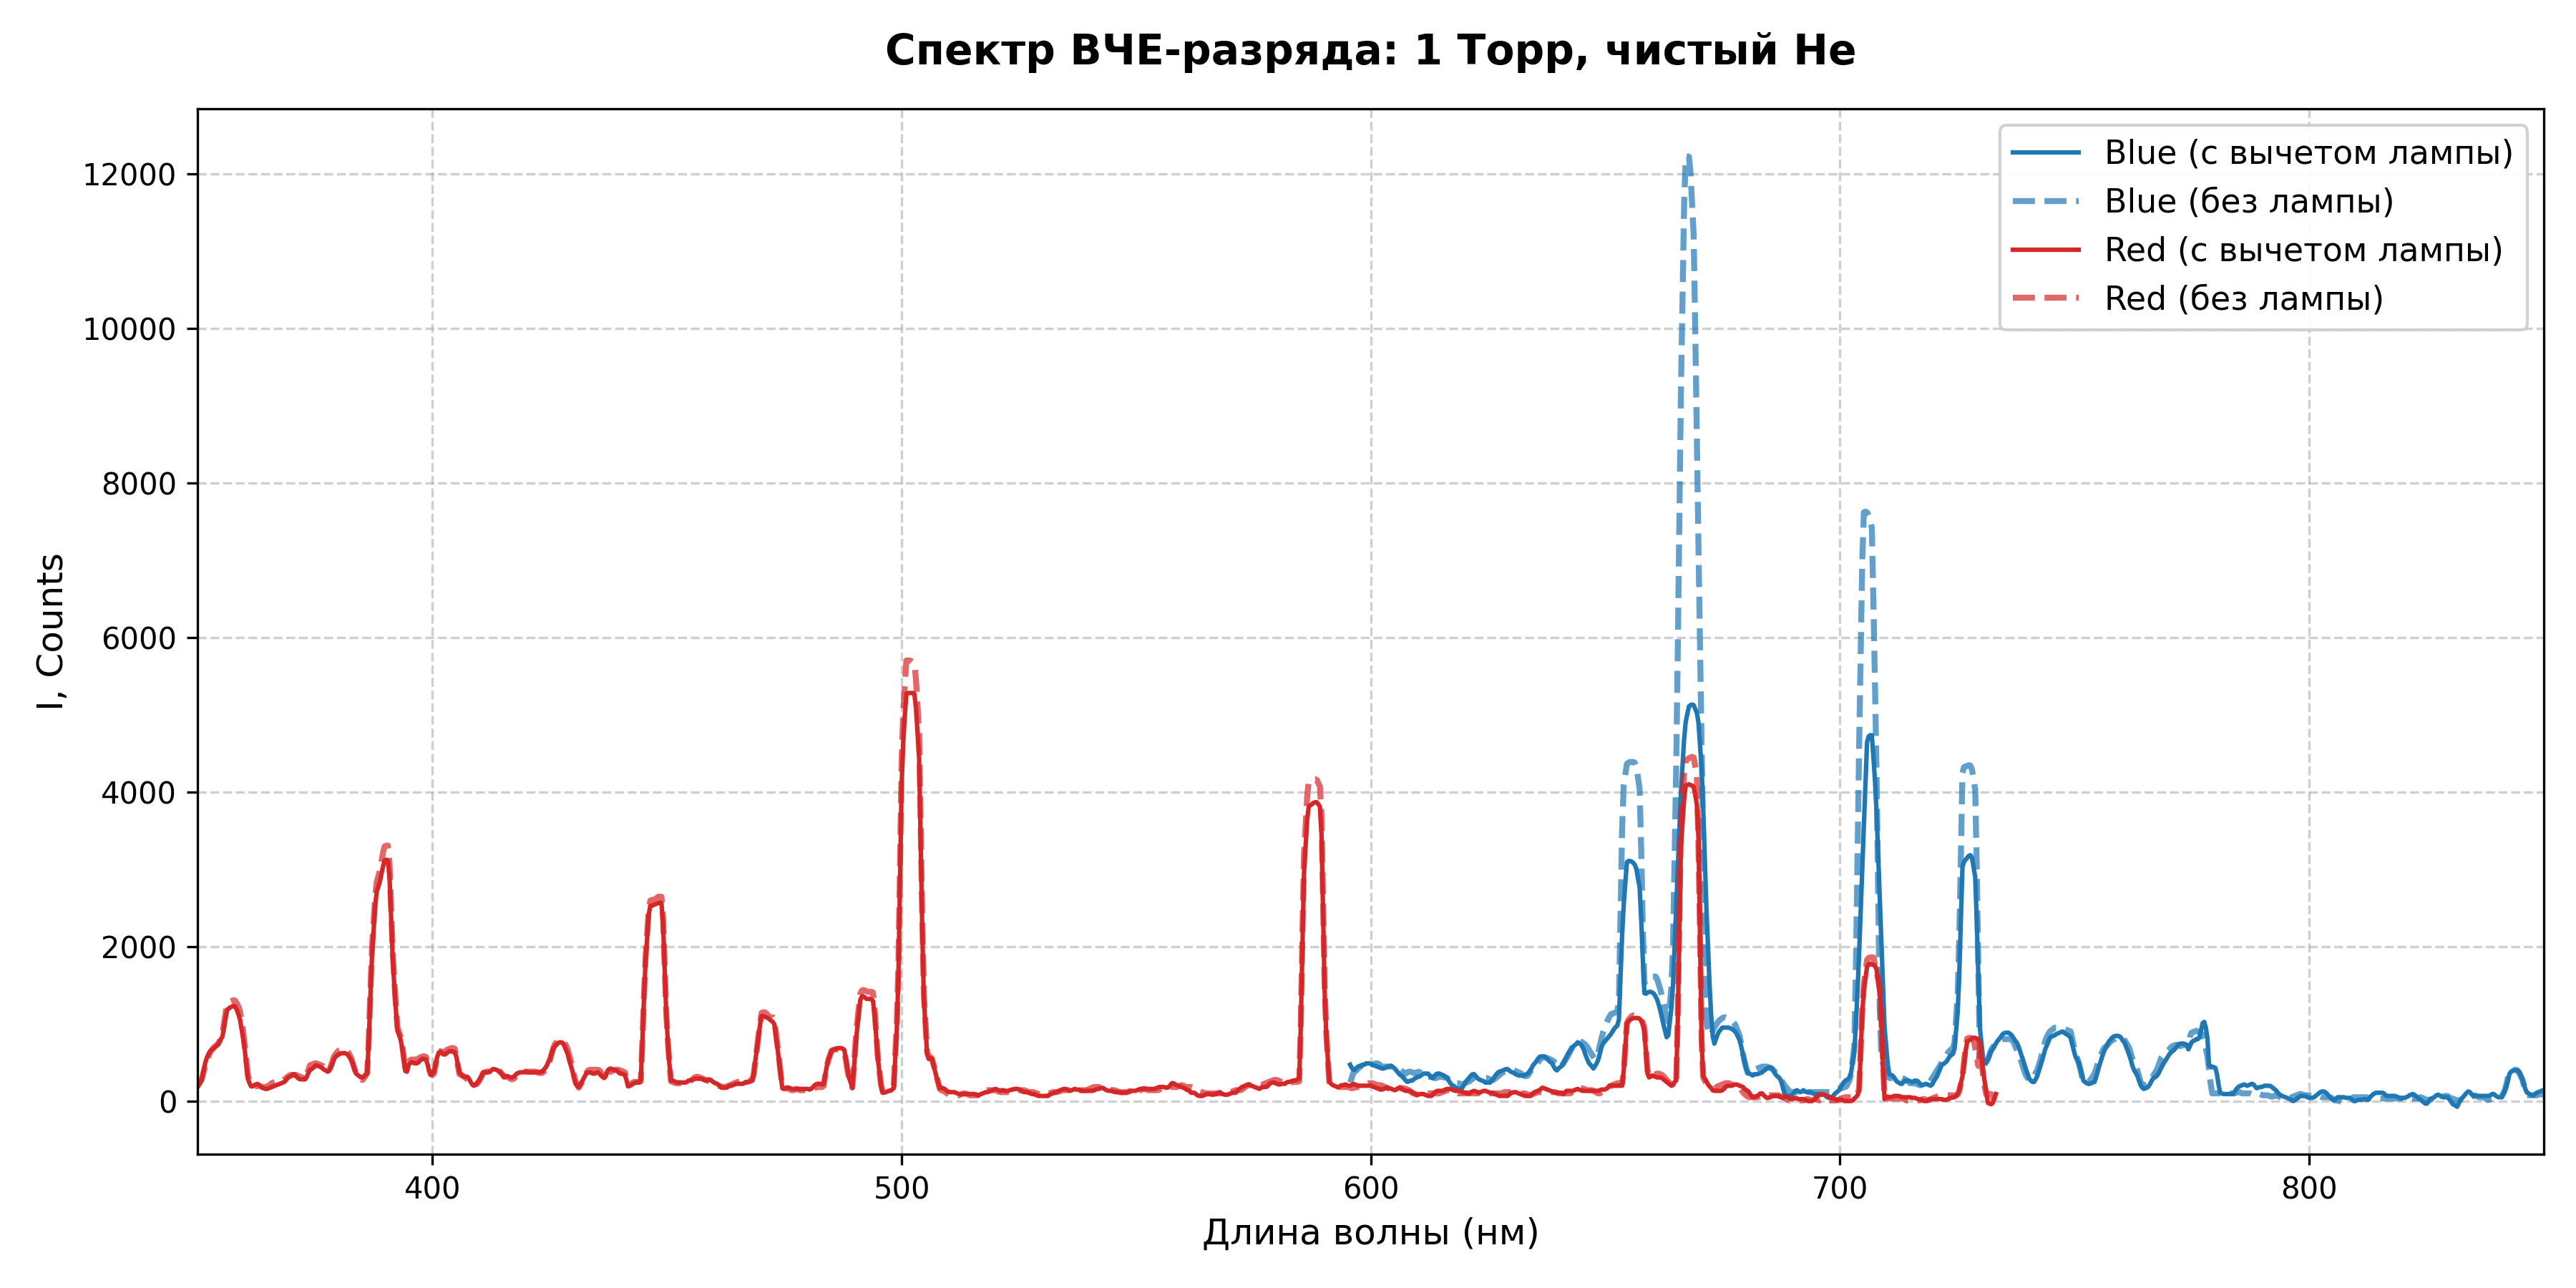
\includegraphics[width=\linewidth]{transp_He_1torr.png}
      {\scriptsize чистый He, 1~Торр: сплошные --- (разряд + лампа) $-$ лампа,
      штриховые --- только разряд}
    \end{column}
    \begin{column}{0.4\textwidth}
      \small
      Если плазма прозрачна: $S_\text{р+л} - S_\text{л} = S_\text{р}$
      \begin{itemize}
        \item Master: совпадение во всех 4 режимах, провалов нет
        \item Slave: дефицит на ярких линиях He
      \end{itemize}
      \textbf{Это эффект прибора:}
      \begin{itemize}
        \item та же линия 668~нм на Master дефицита не имеет
        \item сигнал с лампой «упирается» в один уровень $\approx 12$--14,5 тыс.
              --- насыщение детектора
      \end{itemize}
      $\Rightarrow$ поглощения нет в пределах $\lesssim 10\%$, плазма оптически тонкая
    \end{column}
  \end{columns}
\end{frame}

% ===============================================================
\section{Выводы}
% ===============================================================

\begin{frame}{Выводы}
  \small
  \begin{enumerate}
    \item \textbf{ЭПП:} профиль $B(z)$ имеет максимум, который с ростом давления
          сдвигается к окну: $\Nt$ $13{,}1 \to 4{,}8$~см, Ar $10{,}8 \to 2{,}4$~см;
          в Ar максимум ближе. Тенденции совпадают с пособием (рис.~6.8).
    \item Пробег (1,6--11~м) $\gg$ длины трубки: максимум задаётся
          \textbf{рассеянием} и уходом электронов на стенку; оценка $z_R$
          даёт правильный порядок и отношение Ar/$\Nt$.
    \item \textbf{Монте-Карло} совпадает с опытом при 1~Торр, но почти не
          реагирует на давление --- вероятно, из-за входных данных расчёта.
    \item \textbf{ВЧЕ-разряд:} при 1~Торр $\alpha$-форма, при 3,5--3,9~Торр
          переход в $\gamma$-форму, $P_m L = 13$--$14{,}5$~Торр$\cdot$см ---
          согласуется с примером методички для технического He.
    \item \textbf{Спектры:} полосы $\Nt$, $\mathrm{N_2^+}$, OH в обоих газах;
          азот преобладает при $P_m \gtrsim 2{,}5$--5~Торр, $x_{\Nt} \sim 1\%$.
    \item \textbf{Плазма оптически прозрачна} в пределах $\lesssim 10\%$.
  \end{enumerate}
  \centering\vspace{0.5em}
  {\large Спасибо за внимание!}
\end{frame}

% ===============================================================
\appendix
\section*{Дополнительно}
% ===============================================================

\begin{frame}{Доп.: выводные окна, газодинамическое окно}
  \centering
  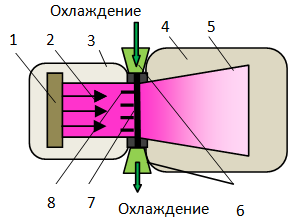
\includegraphics[width=0.27\linewidth]{window_foil.png}\hfill
  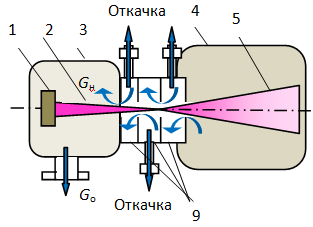
\includegraphics[width=0.27\linewidth]{window_lock.png}\hfill
  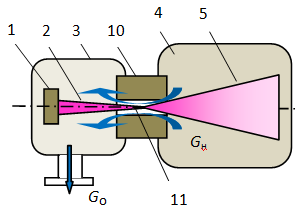
\includegraphics[width=0.27\linewidth]{window_gasdyn.png}

  {\scriptsize фольговое, шлюзовое, газодинамическое (пособие, рис.~6.2)}
  \begin{itemize}
    \item пушке нужен $10^{-5}$~Торр, плазме --- 1--10~Торр
    \item газодинамическое окно: узкий канал в графите; пучок нагревает газ
          в канале, горячий газ протекает хуже:
          $G_\text{х}/G_\text{г} \approx \sqrt{2T_\text{г}/T_\text{х} - 1}$
    \item графит сублимирует (канал не затягивается расплавом), две вставки
          с промежуточной откачкой --- как двухступенчатый шлюз
  \end{itemize}
\end{frame}

\begin{frame}{Доп.: границы применимости формулы Бете--Блоха}
  \[
    -\frac{dE}{dl} = \frac{2\pi N_A e^4 Z\rho}{A\,E}\ln\frac{bE}{I_\text{ср}}
  \]
  \begin{enumerate}
    \item при энергиях, сравнимых с энергиями связи, возбуждаются не все
          оболочки: $I_\text{ср} = I_\text{ср}(E)$
    \item при $bE/I_\text{ср} \le 1$ логарифм отрицателен: $dE/dl > 0$,
          электрон «набирал бы» энергию
    \item при малых $E$ потери идут крупными дискретными порциями, движение
          диффузионное --- модель непрерывного замедления неприменима
  \end{enumerate}
  Нижняя граница $E \approx 150$~эВ; на ней обрываются траектории в
  расчёте Монте-Карло.
\end{frame}

\begin{frame}{Доп.: как отделить свечение плазмы от люминесценции кварца}
  \begin{columns}[T]
    \begin{column}{0.42\textwidth}
      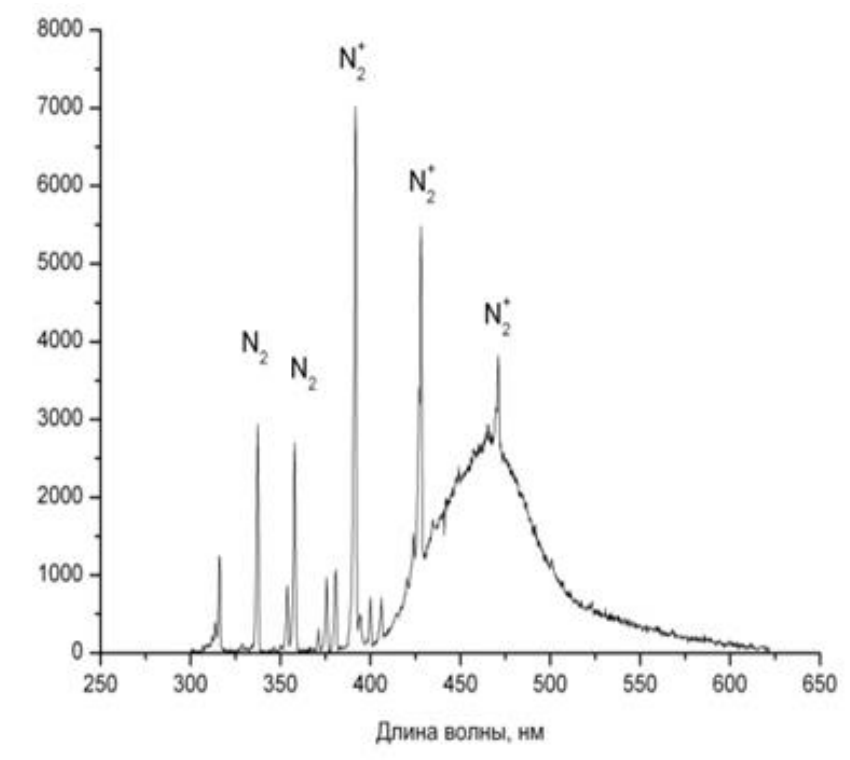
\includegraphics[width=\linewidth]{book_fig4_11_quartz.png}
      {\scriptsize ЭПП азота на фоне люминесценции кварца (пособие, рис.~4.11)}
    \end{column}
    \begin{column}{0.55\textwidth}
      \begin{itemize}
        \item \textbf{по спектру:} плазма --- линии и полосы, кварц ---
              непрерывный горб 400--600~нм; континуум вычитается
              базовой линией; для снимков --- узкополосный фильтр
        \item \textbf{контрольный опыт:} отдельно спектр плазмы и спектр
              люминесценции материала
        \item \textbf{инженерно:} трубка большего диаметра или сжатие
              пучка продольным магнитным полем
      \end{itemize}
    \end{column}
  \end{columns}
\end{frame}

\begin{frame}{Доп.: откуда OH; амбиполярная диффузия}
  \textbf{OH (306--310~нм)}
  \begin{itemize}
    \item камера откачивается только форвакуумным насосом ($\sim 0{,}1$~Торр);
          вода остаётся на стенках и выделяется при нагреве разрядом
    \item в разряде молекулы воды разбиваются на H и OH, возбуждённый OH
          светится около 308~нм
    \item в чистом He при 5~Торр это самый яркий пик спектра
  \end{itemize}
  \medskip
  \textbf{Амбиполярная диффузия}
  \begin{itemize}
    \item электроны быстрее ионов, возникает поле, которое тормозит
          электроны и ускоряет ионы; уходят на стенку вместе:
          $D_a \approx D_i(1 + T_e/T_i)$
    \item в ЭПП выполняется всегда ($n_e \gg 10^4$~см$^{-3}$); радиус трубки
          задаёт время ухода зарядов $\tau \sim R^2/D_a$
  \end{itemize}
\end{frame}

\end{document}
